\section{Durchführung}

    Im Folgenden wird die Durchführung der Messung der Energieverteilung und der Franck-Hertz-Kurve erläutert.\\
    Es ist das folgende Schaltbild gegeben.
    \begin{figure}[H]
        \centering
        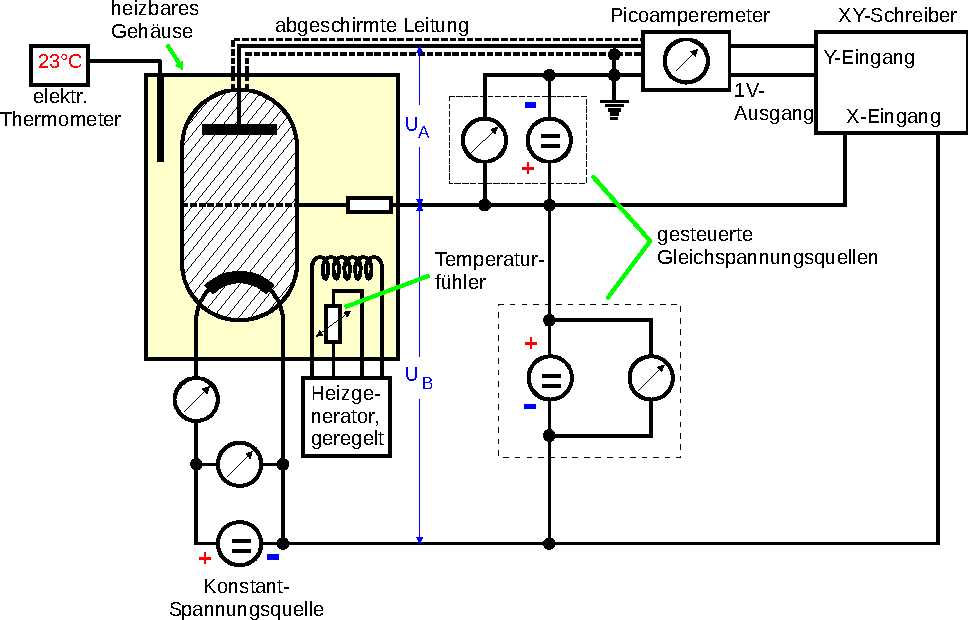
\includegraphics[width=\textwidth]{content/img/Abb_6.pdf}
        \caption{Schaltbild zur Messung der Energieverteilung und der Franck-Hertz-Kurve. \cite{versuchsanleitung}}
        \label{fig:schaltbild}
    \end{figure}
    Zusätzlich zum Aufbau in \autoref{fig:aufbau} aus \autoref{sec:grundprinzip}
    werden ein Heizgenerator mit einem Thermometer,
    Gleichspannungsquellen,
    ein Picoamperemeter
    und ein XY-Schreiber zum Aufzeichnen der Kurven benötigt.\\
    \\
    Die Beschleunigungsspannung kann in einem Bereich von $\SI{0}{\volt} \leq U_\text{B} \leq \SI{60}{\volt}$ variiert werden,
    die Bremsspannung in einem Bereich von $\SI{0}{\volt} \leq U_\text{A} \leq \SI{11}{\volt}$.\\
    % TODO Wie „eingestellt“? 🤔
    Zu Beginn muss der XY-Schreiber eingestellt werden,
    indem die Beschleunigungsspannung an den X-Eingang,
    und die Bremsspannung, welche proportional zum Auffängerstrom ist,
    an den Y-Eingang angelegt wird.\\
    \\
    Nun wird zur Messung der Energieverteilung eine konstante Beschleunigungsspannung von $U_\text{B} = \SI{11}{\volt}$ eingestellt
    und die Bremsspannung langsam erhöht.
    Der XY-Schreiber zeichnet den Verlauf des Auffängerstroms in Abhängigkeit von der Bremsspannung auf.\\
    Diese Messung wird einmal für eine Temperatur von etwa $\SI{20}{\celsius}$
    und ein zweites Mal für eine Temperatur von $\SI{140}{\celsius}$ bis $\SI{160}{\celsius}$ durchgeführt,
    wobei der XY-Schreiber gegebenenfalls neu kallibriert werden muss,
    damit das richtige Y-Intervall dargestellt wird.
    Die Temperatur kann mithilfe des Heizgenerators eingestellt werden.\\
    Nun wird noch die X-Skalierung auf dem Blatt notiert,
    indem die Bremsspannung langsam verändert wird und in $\SI{1}{\volt}$-Schritten Markierungen gesetzt werden.\\
    \\
    Anschließend wird die Franck-Hertz-Kurve gemessen.
    Dazu wird eine konstante Bremsspannung von $U_\text{A} = \SI{1}{\volt}$ eingestellt.
    Stattdessen wird nun die Beschleunigungsspannung auf der X-Achse dargestellt.
    Mithilfe des Heizgenerators wird eine möglichst konstante Temperatur eingestellt.
    Es werden zwei Kurven in einem Temperaturintervall von $T = [\SI{160}{\celsius}, \SI{200}{\celsius}]$ aufgenommen.\\
    Auch hier wird eine X-Skala in $\SI{1}{\volt}$-Schritten hinzugefügt.
